\newpage

\section{Síntesis y Análisis de Temporización (Timing)}

\subsection{Reportes de Vivado}
Una vez validado el diseño a nivel funcional mediante simulación, se procedió a su síntesis e implementación en Vivado con el objetivo de evaluar el costo en recursos y su comportamiento temporal sobre FPGA. Los reportes generados por la herramienta permitieron analizar la utilización de LUTs, registros, memoria embebida y rutas críticas, así como también verificar si el sistema cumplía con las restricciones de reloj planteadas.

Este análisis no solo permitió comprobar si el diseño era sintetizable, sino también detectar puntos sensibles en la implementación. En particular, fue importante estudiar cómo impactaban sobre el timing la interconexión entre etapas del pipeline, la lógica de forwarding, la unidad de hazards y el acceso a memorias. También se revisaron advertencias metodológicas y de temporización que surgieron durante el flujo de implementación, ya que varias de ellas ayudaron a identificar zonas del diseño que requerían una revisión más cuidadosa.

Otro aspecto que debió considerarse fue la correspondencia entre la memoria inferida o instanciada y la latencia asumida por el pipeline. Durante el desarrollo, una de las dificultades más importantes estuvo asociada justamente a la lectura de memoria de datos, ya que una discrepancia entre la latencia esperada y la configurada en el bloque de memoria podía desplazar los datos un ciclo completo y producir resultados incorrectos en la etapa de escritura.



\subsection{Identificación del Camino Crítico y Análisis Temporal}

Para la validación temporal del diseño se utilizó un reloj interno generado mediante el bloque \texttt{Clocking Wizard}, a partir del reloj base de la placa. Este mismo se tuvo que utilizar dado que en las primeras implementaciones no se pudo utilizar el reloj base porque no cumplía con los requisitos de timing. Durante las distintas etapas del desarrollo se trabajó con varias configuraciones de frecuencia, observándose que, a medida que se incorporaban nuevas funcionalidades al procesador ---como lógica adicional de control, señales de depuración, mecanismos de volcado por UART y mayor interconexión entre módulos---, el cierre temporal se volvía más exigente. En consecuencia, fue necesario reducir progresivamente la frecuencia de operación hasta alcanzar una configuración estable de \textbf{72 MHz}, adoptada finalmente para el funcionamiento del sistema.

Este comportamiento es esperable en un diseño de este tipo, ya que el agregado de nuevas señales y caminos de control no sólo incrementa la profundidad lógica de ciertos recorridos, sino también el costo de ruteo y el \textit{fanout} de señales críticas. Por ese motivo, la frecuencia máxima práctica no quedó determinada únicamente por la lógica funcional del pipeline, sino también por la complejidad de integración alcanzada en la implementación final.

\begin{figure}[H]
    \centering
    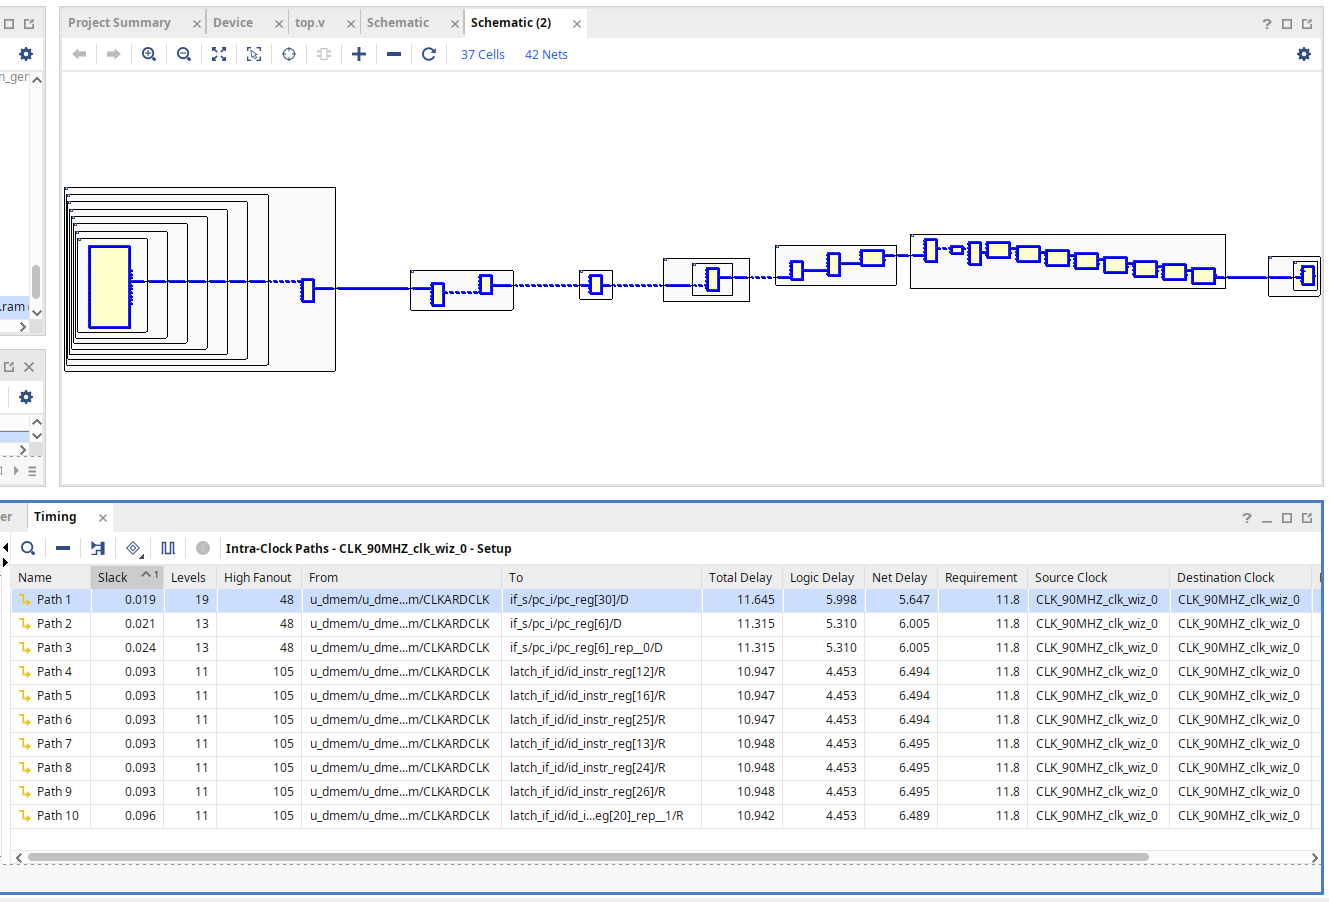
\includegraphics[width=\textwidth]{img/camino.png}
    \caption{Camino crítico identificado por Vivado, comprometiendo principalmente a las etapas MEM, WB, ID e IF del pipeline.}
    \label{fig:camino_critico}
\end{figure}

El análisis del camino crítico mostró que el retardo más exigente del sistema no se concentra en un único bloque aislado, sino en un recorrido que enlaza varias partes relevantes de la arquitectura. De acuerdo con el esquema del camino crítico reportado por Vivado, dicho recorrido parte desde la memoria de datos, atraviesa la lógica de selección del dato de escritura de la etapa de \textit{write back}, interactúa con el banco de registros y la etapa de decodificación (\texttt{regfile32}, \texttt{id\_stage}) y finalmente alcanza la lógica de actualización del contador de programa y registros vinculados a la etapa de \textit{instruction fetch} (\texttt{pc} e \texttt{if\_id\_reg}).

Desde el punto de vista arquitectónico, esto implica que en el camino crítico intervienen principalmente las etapas \textbf{MEM}, \textbf{WB}, \textbf{ID} e \textbf{IF}. En otras palabras, el dato leído desde memoria debe propagarse hasta la lógica de escritura de registros, afectar señales utilizadas durante la decodificación y participar luego en la lógica que condiciona la actualización del PC y de los registros inter-etapa. Esta extensión del recorrido explica por qué el retardo total no depende únicamente de operadores aritméticos o multiplexores, sino también de la propagación a través de varios módulos conectados entre sí.

\begin{figure}[H]
    \centering
    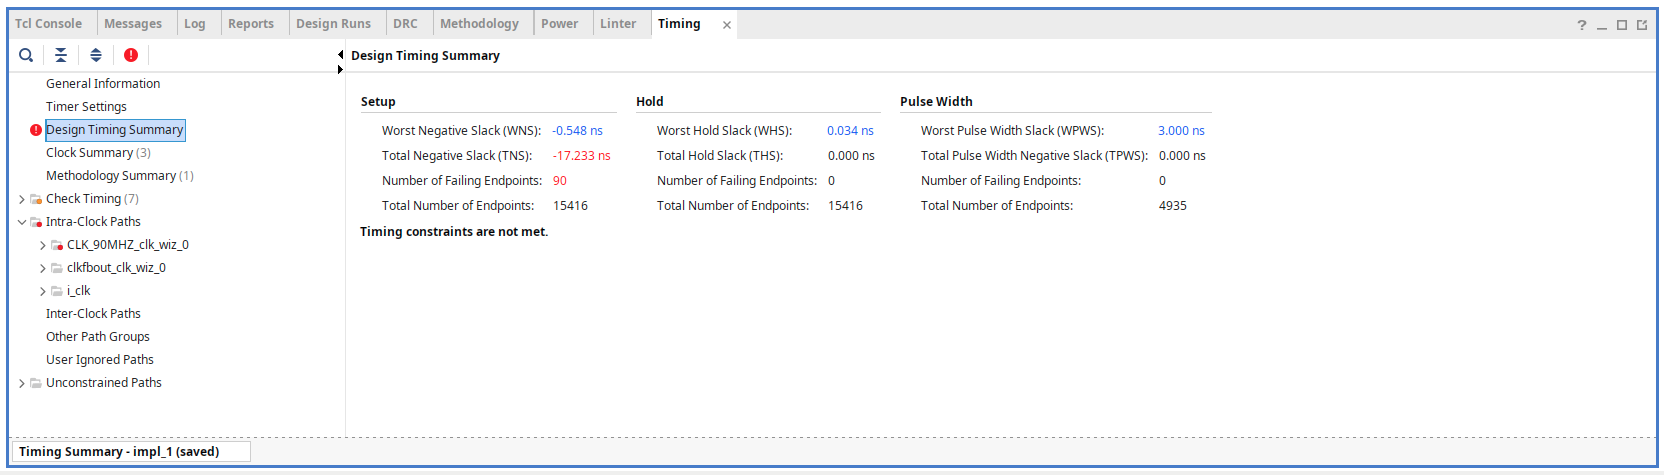
\includegraphics[width=\textwidth]{img/summary.png}
    \caption{Resumen temporal de implementación en una configuración que no alcanzaba a cumplir las restricciones impuestas. Se observa una violación de \textit{setup}, con \textit{Worst Negative Slack} negativo y múltiples endpoints en falla.}
    \label{fig:timing_summary}
\end{figure}

\begin{figure}[H]
    \centering
    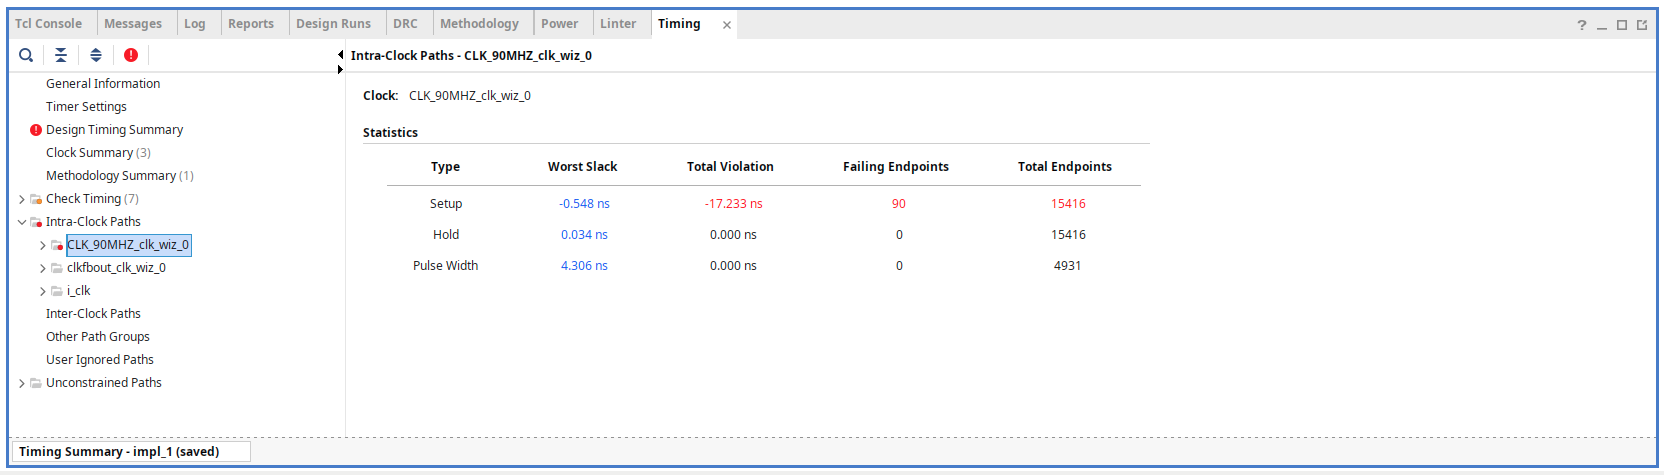
\includegraphics[width=\textwidth]{img/intra-clock.png}
    \caption{Resumen de caminos \textit{intra-clock}. Se observa que las violaciones temporales se concentraban dentro de un mismo dominio de reloj.}
    \label{fig:intra_clock_paths}
\end{figure}

Los reportes mostraron que el retardo total del camino crítico se reparte de manera comparable entre \textit{logic delay} y \textit{net delay}. Esto indica que el problema no se debe sólo a la profundidad combinacional, sino también al costo de interconexión física entre bloques, aspecto particularmente importante cuando el diseño crece en complejidad y el ruteo comienza a tener un peso similar al de la propia lógica.

\begin{figure}[H]
    \centering
    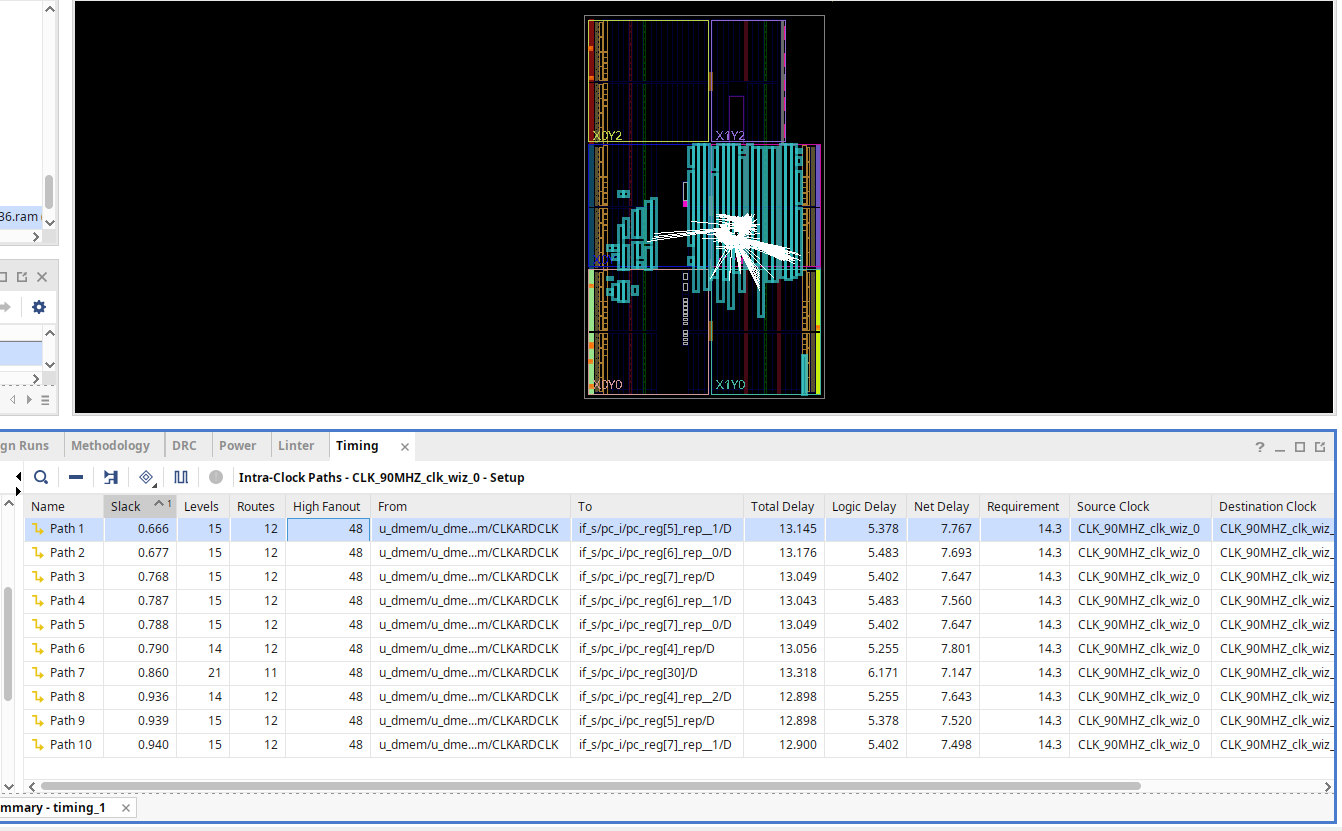
\includegraphics[width=\textwidth]{img/timing_routing.png}
    \caption{Visualización del ruteo.}
    \label{fig:timing_routing72mhz}
\end{figure}

\begin{figure}[H]
    \centering
    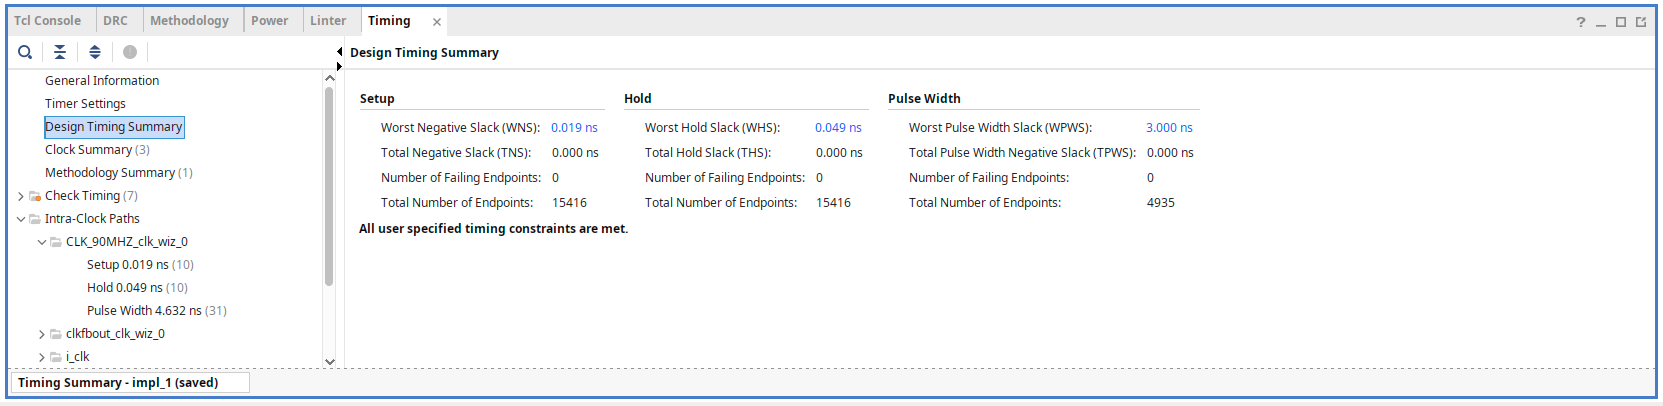
\includegraphics[width=\textwidth]{img/timing_summary.png}
    \caption{Resumen temporal de la implementación final. Se verifica que todas las restricciones temporales especificadas se cumplen, con \textit{Worst Negative Slack} positivo y sin \textit{endpoints} en falla.}
    \label{fig:timing_summary_72mhz}
\end{figure}

En este contexto, la selección final de \textbf{72 MHz} representó un compromiso razonable entre rendimiento y robustez temporal. Esta configuración permitió conservar el comportamiento correcto del pipeline, la interacción con memorias y el funcionamiento de la unidad de depuración, manteniendo un margen temporal más adecuado para la implementación completa del sistema.




% \subsection{Identificación del Camino Crítico y Skew}
% En una arquitectura segmentada, el objetivo principal del pipeline es aumentar el rendimiento permitiendo que varias instrucciones avancen en paralelo. Sin embargo, el período mínimo de reloj sigue estando condicionado por el camino combinacional más largo del diseño, es decir, por el llamado \textit{camino crítico}.

% En este trabajo, el camino crítico se encontró asociado a la interconexión entre registros del pipeline y lógica de procesamiento involucrada en la ejecución de instrucciones, particularmente en los recorridos que incluyen \textbf{cálculo de resultados, selección de datos mediante multiplexores y escritura posterior en registros}. Según la configuración sintetizada, estos caminos pueden involucrar la salida de memoria, los registros intermedios del pipeline, la lógica de selección del dato de escritura y su retorno hacia el banco de registros.

% Este resultado es coherente con la experiencia de desarrollo, ya que una parte importante de la depuración se centró precisamente en comprender cómo se propagaban los datos entre etapas y en qué ciclo exacto quedaban disponibles. La interacción entre memorias, registros de pipeline y lógica de selección resultó ser un punto especialmente sensible, tanto desde lo funcional como desde lo temporal.

% Junto con el camino crítico, también resulta relevante considerar el \textit{clock skew}, es decir, la diferencia de tiempo con la que el flanco de reloj llega a distintos registros del circuito. Aunque este efecto forma parte normal de cualquier implementación física, su influencia se vuelve más importante a medida que se exige una frecuencia de operación mayor.

% Si el margen temporal disponible es demasiado reducido, el skew puede contribuir a violaciones de \textit{setup time}, impidiendo que una señal llegue y se estabilice correctamente antes del siguiente flanco de reloj. Por eso, no alcanza con que la lógica sea funcionalmente correcta: también debe cumplir con las restricciones temporales impuestas por la tecnología y el ruteo físico sobre FPGA.

% \subsection{Determinación de la Frecuencia Óptima}
% A partir de los resultados de síntesis e implementación, se buscó determinar una frecuencia de operación que ofreciera un equilibrio entre rendimiento y robustez temporal. Para ello, se analizaron los valores de \textit{slack} obtenidos en los reportes de timing, procurando mantener un margen positivo que garantizara un funcionamiento confiable del procesador.

% Durante el desarrollo, se trabajó principalmente con relojes del orden de decenas de MHz, y se evaluó también el comportamiento del sistema frente a distintas configuraciones de frecuencia. Este análisis resultó importante no solo para validar la CPU en sí, sino también para asegurar la correcta interacción con módulos auxiliares como la UART y las memorias embebidas.

% En este contexto, se observó que no siempre la máxima frecuencia teórica resultaba ser la opción más conveniente para la validación completa del sistema. En varias etapas del proyecto fue preferible priorizar una configuración estable y repetible, que permitiera verificar correctamente la ejecución del pipeline, el intercambio UART y la depuración interna, antes que exigir el límite absoluto de operación.

% Por lo tanto, la frecuencia de trabajo adoptada se definió considerando no solo el cumplimiento de timing, sino también la estabilidad global del sistema, la reproducibilidad de las pruebas y la correcta integración entre todos los módulos del procesador.
